\documentclass[11pt,a4paper,]{article}
\usepackage{lmodern}

\usepackage{amssymb,amsmath}
\usepackage{ifxetex,ifluatex}
\usepackage{fixltx2e} % provides \textsubscript
\ifnum 0\ifxetex 1\fi\ifluatex 1\fi=0 % if pdftex
  \usepackage[T1]{fontenc}
  \usepackage[utf8]{inputenc}
\else % if luatex or xelatex
  \usepackage{unicode-math}
  \defaultfontfeatures{Ligatures=TeX,Scale=MatchLowercase}
\fi
% use upquote if available, for straight quotes in verbatim environments
\IfFileExists{upquote.sty}{\usepackage{upquote}}{}
% use microtype if available
\IfFileExists{microtype.sty}{%
\usepackage[]{microtype}
\UseMicrotypeSet[protrusion]{basicmath} % disable protrusion for tt fonts
}{}
\PassOptionsToPackage{hyphens}{url} % url is loaded by hyperref
\usepackage[unicode=true]{hyperref}
\hypersetup{
            pdftitle={M4 Competition: FFORMS framework},
            pdfborder={0 0 0},
            breaklinks=true}
\urlstyle{same}  % don't use monospace font for urls
\usepackage{geometry}
\geometry{a4paper, text={16cm,24cm}}
\usepackage[style=authoryear-comp,]{biblatex}
\addbibresource{references.bib}
\usepackage{color}
\usepackage{fancyvrb}
\newcommand{\VerbBar}{|}
\newcommand{\VERB}{\Verb[commandchars=\\\{\}]}
\DefineVerbatimEnvironment{Highlighting}{Verbatim}{commandchars=\\\{\}}
% Add ',fontsize=\small' for more characters per line
\usepackage{framed}
\definecolor{shadecolor}{RGB}{248,248,248}
\newenvironment{Shaded}{\begin{snugshade}}{\end{snugshade}}
\newcommand{\KeywordTok}[1]{\textcolor[rgb]{0.13,0.29,0.53}{\textbf{#1}}}
\newcommand{\DataTypeTok}[1]{\textcolor[rgb]{0.13,0.29,0.53}{#1}}
\newcommand{\DecValTok}[1]{\textcolor[rgb]{0.00,0.00,0.81}{#1}}
\newcommand{\BaseNTok}[1]{\textcolor[rgb]{0.00,0.00,0.81}{#1}}
\newcommand{\FloatTok}[1]{\textcolor[rgb]{0.00,0.00,0.81}{#1}}
\newcommand{\ConstantTok}[1]{\textcolor[rgb]{0.00,0.00,0.00}{#1}}
\newcommand{\CharTok}[1]{\textcolor[rgb]{0.31,0.60,0.02}{#1}}
\newcommand{\SpecialCharTok}[1]{\textcolor[rgb]{0.00,0.00,0.00}{#1}}
\newcommand{\StringTok}[1]{\textcolor[rgb]{0.31,0.60,0.02}{#1}}
\newcommand{\VerbatimStringTok}[1]{\textcolor[rgb]{0.31,0.60,0.02}{#1}}
\newcommand{\SpecialStringTok}[1]{\textcolor[rgb]{0.31,0.60,0.02}{#1}}
\newcommand{\ImportTok}[1]{#1}
\newcommand{\CommentTok}[1]{\textcolor[rgb]{0.56,0.35,0.01}{\textit{#1}}}
\newcommand{\DocumentationTok}[1]{\textcolor[rgb]{0.56,0.35,0.01}{\textbf{\textit{#1}}}}
\newcommand{\AnnotationTok}[1]{\textcolor[rgb]{0.56,0.35,0.01}{\textbf{\textit{#1}}}}
\newcommand{\CommentVarTok}[1]{\textcolor[rgb]{0.56,0.35,0.01}{\textbf{\textit{#1}}}}
\newcommand{\OtherTok}[1]{\textcolor[rgb]{0.56,0.35,0.01}{#1}}
\newcommand{\FunctionTok}[1]{\textcolor[rgb]{0.00,0.00,0.00}{#1}}
\newcommand{\VariableTok}[1]{\textcolor[rgb]{0.00,0.00,0.00}{#1}}
\newcommand{\ControlFlowTok}[1]{\textcolor[rgb]{0.13,0.29,0.53}{\textbf{#1}}}
\newcommand{\OperatorTok}[1]{\textcolor[rgb]{0.81,0.36,0.00}{\textbf{#1}}}
\newcommand{\BuiltInTok}[1]{#1}
\newcommand{\ExtensionTok}[1]{#1}
\newcommand{\PreprocessorTok}[1]{\textcolor[rgb]{0.56,0.35,0.01}{\textit{#1}}}
\newcommand{\AttributeTok}[1]{\textcolor[rgb]{0.77,0.63,0.00}{#1}}
\newcommand{\RegionMarkerTok}[1]{#1}
\newcommand{\InformationTok}[1]{\textcolor[rgb]{0.56,0.35,0.01}{\textbf{\textit{#1}}}}
\newcommand{\WarningTok}[1]{\textcolor[rgb]{0.56,0.35,0.01}{\textbf{\textit{#1}}}}
\newcommand{\AlertTok}[1]{\textcolor[rgb]{0.94,0.16,0.16}{#1}}
\newcommand{\ErrorTok}[1]{\textcolor[rgb]{0.64,0.00,0.00}{\textbf{#1}}}
\newcommand{\NormalTok}[1]{#1}
\usepackage{longtable,booktabs}
% Fix footnotes in tables (requires footnote package)
\IfFileExists{footnote.sty}{\usepackage{footnote}\makesavenoteenv{long table}}{}
\IfFileExists{parskip.sty}{%
\usepackage{parskip}
}{% else
\setlength{\parindent}{0pt}
\setlength{\parskip}{6pt plus 2pt minus 1pt}
}
\setlength{\emergencystretch}{3em}  % prevent overfull lines
\providecommand{\tightlist}{%
  \setlength{\itemsep}{0pt}\setlength{\parskip}{0pt}}
\setcounter{secnumdepth}{5}

% set default figure placement to htbp
\makeatletter
\def\fps@figure{htbp}
\makeatother


\title{M4 Competition: FFORMS framework}

%% MONASH STUFF

%% CAPTIONS
\RequirePackage{caption}
\DeclareCaptionStyle{italic}[justification=centering]
 {labelfont={bf},textfont={it},labelsep=colon}
\captionsetup[figure]{style=italic,format=hang,singlelinecheck=true}
\captionsetup[table]{style=italic,format=hang,singlelinecheck=true}

%% FONT
\RequirePackage{bera}
\RequirePackage{mathpazo}

%% HEADERS AND FOOTERS
\RequirePackage{fancyhdr}
\pagestyle{fancy}
\rfoot{\Large\sffamily\raisebox{-0.1cm}{\textbf{\thepage}}}
\makeatletter
\lhead{\textsf{\expandafter{\@title}}}
\makeatother
\rhead{}
\cfoot{}
\setlength{\headheight}{15pt}
\renewcommand{\headrulewidth}{0.4pt}
\renewcommand{\footrulewidth}{0.4pt}
\fancypagestyle{plain}{%
\fancyhf{} % clear all header and footer fields
\fancyfoot[C]{\sffamily\thepage} % except the center
\renewcommand{\headrulewidth}{0pt}
\renewcommand{\footrulewidth}{0pt}}

%% MATHS
\RequirePackage{bm,amsmath}
\allowdisplaybreaks

%% GRAPHICS
\RequirePackage{graphicx}
\setcounter{topnumber}{2}
\setcounter{bottomnumber}{2}
\setcounter{totalnumber}{4}
\renewcommand{\topfraction}{0.85}
\renewcommand{\bottomfraction}{0.85}
\renewcommand{\textfraction}{0.15}
\renewcommand{\floatpagefraction}{0.8}

%\RequirePackage[section]{placeins}

%% SECTION TITLES
\RequirePackage[compact,sf,bf]{titlesec}
\titleformat{\section}[block]
  {\fontsize{15}{17}\bfseries\sffamily}
  {\thesection}
  {0.4em}{}
\titleformat{\subsection}[block]
  {\fontsize{12}{14}\bfseries\sffamily}
  {\thesubsection}
  {0.4em}{}
\titlespacing{\section}{0pt}{*5}{*1}
\titlespacing{\section}{0pt}{*2}{*0.2}


%% TITLE PAGE
\def\Date{\number\day}
\def\Month{\ifcase\month\or
 January\or February\or March\or April\or May\or June\or
 July\or August\or September\or October\or November\or December\fi}
\def\Year{\number\year}

\makeatletter
\def\wp#1{\gdef\@wp{#1}}\def\@wp{??/??}
\def\jel#1{\gdef\@jel{#1}}\def\@jel{??}
\def\showjel{{\large\textsf{\textbf{JEL classification:}}~\@jel}}
\def\nojel{\def\showjel{}}
\def\addresses#1{\gdef\@addresses{#1}}\def\@addresses{??}
\def\cover{{\sffamily\setcounter{page}{0}
        \thispagestyle{empty}%
        \vspace*{-2cm}
        \centerline{\raisebox{-1.8cm}{
\includegraphics[width=5cm]{MBSportrait}}\hspace*{9cm} ISSN 1440-771X}\vspace{0.99cm}
        \begin{center}\Large
        Department of Econometrics and Business Statistics\\[.5cm]
        \scriptsize http://business.monash.edu/econometrics-and-business-statistics/research/publications
        \end{center}\vspace{2cm}
        \begin{center}
        \fbox{\parbox{14cm}{\begin{onehalfspace}\centering\Huge\vspace*{0.3cm}
                \textsf{\textbf{\expandafter{\@title}}}\vspace{1cm}\par
                \LARGE\@author\end{onehalfspace}
        }}
        \end{center}
        \vfill
                \begin{center}\Large
                \Month~\Year\\[1cm]
                Working Paper \@wp
        \end{center}}}
\def\pageone{{\sffamily
        \newpage%\blankpage
        \thispagestyle{empty}
        \vbox to 23cm{
        \raggedright\baselineskip=1.2cm
     {\fontsize{24.88}{30}\sffamily\textbf{\expandafter{\@title}}}
        \vspace{2cm}\par
        \hspace{1cm}\parbox{14cm}{\sffamily\large\@addresses}\vspace{1cm}\vfill
        \hspace{1cm}{\large\Date~\Month~\Year}\\[1cm]
        \hspace{1cm}\showjel\vss}}}
\def\blindtitle{{\sffamily
     \thispagestyle{plain}\raggedright\baselineskip=1.2cm
     {\fontsize{24.88}{30}\sffamily\textbf{\expandafter{\@title}}}\vspace{1cm}\par
        }}
\def\titlepage{{\cover\newpage\setstretch{1}\pageone\newpage\blindtitle}}

\def\blind{\def\titlepage{{\blindtitle}}\let\maketitle\blindtitle}
\def\titlepageonly{\def\titlepage{{\pageone\end{document}}}}
\def\nocover{\def\titlepage{{\newpage\setstretch{1}\pageone\newpage\blindtitle}}\let\maketitle\titlepage}
\let\maketitle\titlepage
\makeatother

%% SPACING
\RequirePackage{setspace}
\spacing{1.5}

%% LINE AND PAGE BREAKING
\sloppy
\clubpenalty = 10000
\widowpenalty = 10000
\brokenpenalty = 10000
\RequirePackage{microtype}

%% PARAGRAPH BREAKS
\setlength{\parskip}{1.4ex}
\setlength{\parindent}{0em}

%% HYPERLINKS
\RequirePackage{xcolor} % Needed for links
\definecolor{darkblue}{rgb}{0,0,.6}
\RequirePackage{url}

\makeatletter
\@ifpackageloaded{hyperref}{}{\RequirePackage{hyperref}}
\makeatother
\hypersetup{
     citecolor=0 0 0,
     breaklinks=true,
     bookmarksopen=true,
     bookmarksnumbered=true,
     linkcolor=darkblue,
     urlcolor=blue,
     citecolor=darkblue,
     colorlinks=true}

%% KEYWORDS
\newenvironment{keywords}{\par\vspace{0.5cm}\noindent{\sffamily\textbf{Keywords:}}}{\vspace{0.25cm}\par\hrule\vspace{0.5cm}\par}

%% ABSTRACT
\renewenvironment{abstract}{\begin{minipage}{\textwidth}\parskip=1.4ex\noindent
\hrule\vspace{0.1cm}\par{\sffamily\textbf{\abstractname}}\newline}
  {\end{minipage}}


\usepackage[T1]{fontenc}
\usepackage[utf8]{inputenc}

\usepackage[showonlyrefs]{mathtools}
\usepackage[no-weekday]{eukdate}

%% BIBLIOGRAPHY

\makeatletter
\@ifpackageloaded{biblatex}{}{\usepackage[style=authoryear-comp, backend=biber, natbib=true]{biblatex}}
\makeatother
\ExecuteBibliographyOptions{bibencoding=utf8,minnames=1,maxnames=3, maxbibnames=99,dashed=false,terseinits=true,giveninits=true,uniquename=false,uniquelist=false,doi=false, isbn=false,url=true,sortcites=false}

\DeclareFieldFormat{url}{\texttt{\url{#1}}}
\DeclareFieldFormat[article]{pages}{#1}
\DeclareFieldFormat[inproceedings]{pages}{\lowercase{pp.}#1}
\DeclareFieldFormat[incollection]{pages}{\lowercase{pp.}#1}
\DeclareFieldFormat[article]{volume}{\mkbibbold{#1}}
\DeclareFieldFormat[article]{number}{\mkbibparens{#1}}
\DeclareFieldFormat[article]{title}{\MakeCapital{#1}}
\DeclareFieldFormat[article]{url}{}
%\DeclareFieldFormat[book]{url}{}
%\DeclareFieldFormat[inbook]{url}{}
%\DeclareFieldFormat[incollection]{url}{}
%\DeclareFieldFormat[inproceedings]{url}{}
\DeclareFieldFormat[inproceedings]{title}{#1}
\DeclareFieldFormat{shorthandwidth}{#1}
%\DeclareFieldFormat{extrayear}{}
% No dot before number of articles
\usepackage{xpatch}
\xpatchbibmacro{volume+number+eid}{\setunit*{\adddot}}{}{}{}
% Remove In: for an article.
\renewbibmacro{in:}{%
  \ifentrytype{article}{}{%
  \printtext{\bibstring{in}\intitlepunct}}}

\AtEveryBibitem{\clearfield{month}}
\AtEveryCitekey{\clearfield{month}}

\makeatletter
\DeclareDelimFormat[cbx@textcite]{nameyeardelim}{\addspace}
\makeatother
\renewcommand*{\finalnamedelim}{%
  %\ifnumgreater{\value{liststop}}{2}{\finalandcomma}{}% there really should be no funny Oxford comma business here
  \addspace\&\space}
  

\wp{no/yr}
\jel{C10,C14,C22}


\blind



\date{\sf\Date~\Month~\Year}
\makeatletter
 \lfoot{\sf\@date}
\makeatother

%% Any special functions or other packages can be loaded here.
\usepackage{tikz}
\usepackage{algorithm}
\usepackage{algpseudocode}
\usepackage{amsthm}
\usepackage{amsmath,bm}
\usepackage{paralist}
\usepackage{todonotes}
\usepackage{ctable}
\usepackage{multirow}

\def\sectionautorefname{Section}
\captionsetup[figure]{font=small}
\captionsetup[table]{font=small}
\def\var{\text{Var}}
\allowdisplaybreaks
\sloppy

%% LINE AND PAGE BREAKING
\clubpenalty = 4500
\widowpenalty = 4500
\brokenpenalty = 4500


\def\yes{$\checkmark$}

\setlength{\abovedisplayskip}{5pt}
\setlength{\belowdisplayskip}{5pt}
\setlength{\abovedisplayshortskip}{0pt}
\setlength{\belowdisplayshortskip}{0pt}


\usepackage{amsthm}
\newtheorem{theorem}{Theorem}[section]
\newtheorem{lemma}{Lemma}[section]
\newtheorem{corollary}{Corollary}[section]
\newtheorem{proposition}{Proposition}[section]
\newtheorem{conjecture}{Conjecture}[section]
\theoremstyle{definition}
\newtheorem{definition}{Definition}[section]
\theoremstyle{definition}
\newtheorem{example}{Example}[section]
\theoremstyle{definition}
\newtheorem{exercise}{Exercise}[section]
\theoremstyle{remark}
\newtheorem*{remark}{Remark}
\newtheorem*{solution}{Solution}
\begin{document}
\maketitle

\section{Introduction}\label{introduction}

We use Feature-based FORecast-Model Selection (FFORMS) framework
introduced in \autocite{fforms} over the course of the M4 forecasting
competition. The underlying approach involves computing a vector of
features from the time series we will be forecasting which are then used
to select the forecasting model. The model selection process is carried
out using a classification algorithm -- we use the time series features
as inputs, and the best forecasting model as the output. A Random Forest
approach is used to develop the classifier. The classification algorithm
can be built in advance of the forecasting exercise (so it is an
``offline'' procedure). Then, when we have a new time series to
forecast, we can quickly compute its features, use the pre-trained
classification algorithm to identify the best forecasting model, and
produce the required forecasts. Thus, the ``online'' part of our
algorithm requires only feature computation, and the application of a
single forecasting model, with no need to estimate large numbers of
models within a class, or to carry out a computationally-intensive
cross-validation procedure. This framework is implemented in the open
source R package \texttt{seer} and is publicly available on github
(\url{https://github.com/thiyangt/seer}).

\section{FFORMS framework: application to M4 competition
data}\label{fforms-framework-application-to-m4-competition-data}

\begin{figure}[h]
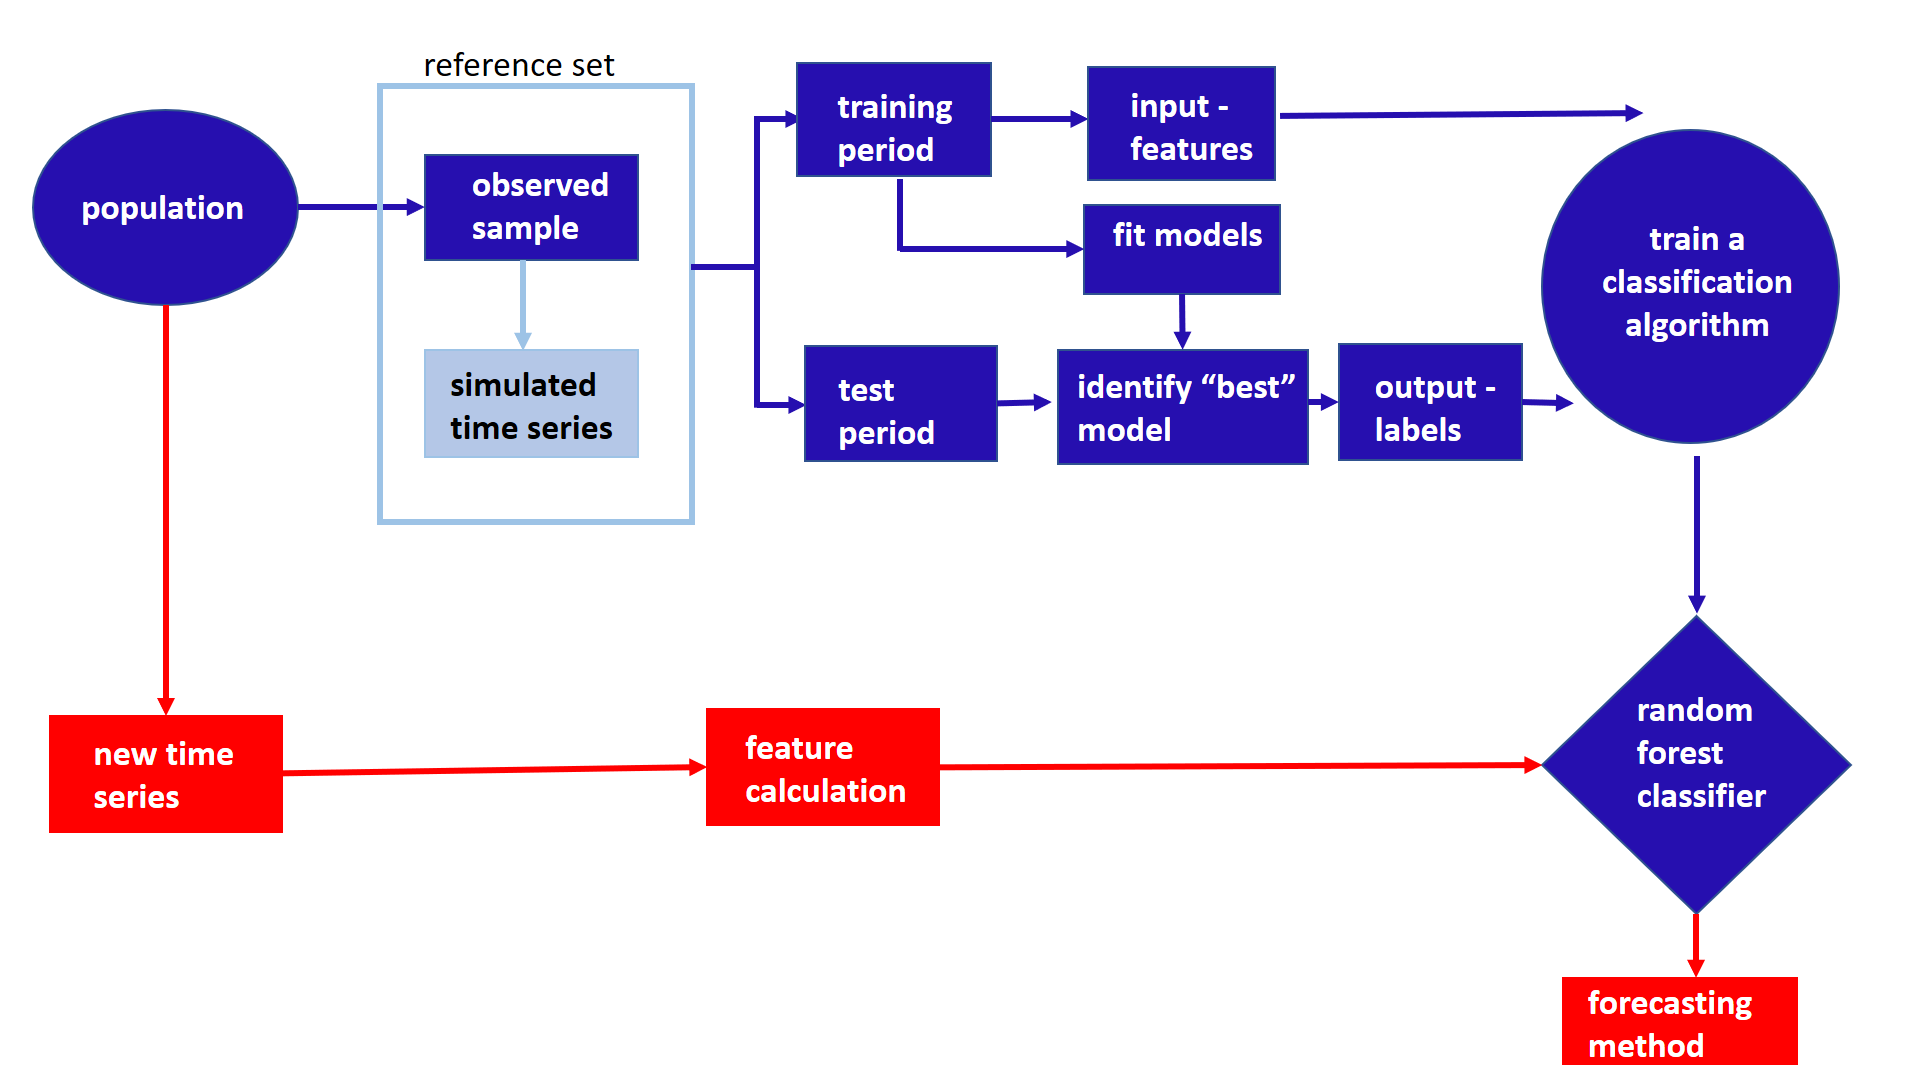
\includegraphics[width=400px]{figures/framework} \caption{FFORMS (Feature-based FORecast-Model Selection) framework. The offline phase is shown in blue and the online phase by red.}\label{fig:framework}
\end{figure}

As shown in \autoref{fig:framework}, the FFORMS framework consists of
two main components: i) \emph{offline phase}, which includes the
development of a classification model and ii) \emph{online phase}, use
the classification model developed in the offline phase to identify
``best'' forecast-model. We develop separate classifiers for yearly,
monthly, quarterly, weekly, daily and hourly series. Now we will
illustrate the implementation of FFORMS framework over the course of the
M4 competition.

\subsection{FFORMS framework: offline
phase}\label{fforms-framework-offline-phase}

\subsubsection{observed sample}\label{observed-sample}

We split the time series in the M4 competition into training set and
test set. The time series in the training set are used as the set of
observed time series. The time series in the test set are used to
evaluate the classification models. Further, for yearly, quarterly and
monthly time series in addition to the time series provided in the M4
competition we used the time series of M1 and M3 competitions. Table
\ref{observedsample} summarizes the number of time series in the
observed sample and the test set in each frequency category.

\begin{table}[!h]
\centering
\caption{Composition of the time series in the observed sample and the test set}
\label{observedsample}
\begin{tabular}{l|rrr|r}
\multirow{2}{*}{Frequency} & \multicolumn{3}{l|}{Observed Sample} &  Test set \\ 
                  &   M1    &    M3   &    M4  &  M4 \\ \hline
  Yearly          &   181    &   645    &   22000   & 1000 \\
  Quarterly       &   203    &    756   &   23000   &  1000\\
  Monthly         &   617    &    1428   &  47000    &  1000\\
  Weekly          &   -    &   -    &   259   & 100 \\
  Daily           &   -    &   -    &   4001   & 226 \\
  Hourly          &   -    &    -   &  350    & 64\\ \hline
\end{tabular}
\end{table}

\subsubsection{simulated time series}\label{simulated-time-series}

As described in \textcite{fforms}, we augment the reference set by
adding multiple time series simulated based on each series in the M4
competition. We use several standard automatic forecasting algorithms to
simulate multiple time series from each series. Table \ref{simulation}
shows the different automatic forecasting algorithms used under each
frequency category. The automated ETS and ARIMA are implemented using
\texttt{ets} and \texttt{auto.arima} functions available in the forecast
package in R \autocite{forecast}. The \texttt{stlf} function in the
forecast package \autocite{forecast} is used to simulate multiple time
series based on multiple seasonal decomposition approach. As shown in
Table \ref{simulation} we fit models to each time series in the M4
competition database from the corresponding algorithm and then simulate
multiple time series from the selected models. Before simulating time
series from daily and hourly series we convert the time series into
multiple seasonal time series (msts) objects. For daily time series with
length less 366 the frequency is set to 7 and if the time series is long
enough to take more than a year (length \textgreater{} 366), the series
is converted to a multiple seasonal time series objects with frequencies
7 and 365.25. For hourly series, if the series length is shorter than
168, frequency is set to 24, if the length of the series is greater than
168 and less than or equals to 8766 only daily and weekly seasonality
are allowed setting the frequencies to 24 and 168. In this experiment
the length of the simulated time series is set to be equal to: length of
the training period specified in the M4 competition + length of the
forecast horizon specified in the competition. For example, the series
with id ``Y13190'' contains a training period of length 835. The length
of the simulated series generated based on this series is equals to 841
(835+6).

\begin{table}[!h]
\centering
\caption{Automatic forecasting algorithms used to simulate time series}
\label{simulation}
\begin{tabular}{lllllll}
 Algorithm & Y & Q & M & W & D &  H \\ \hline
 automated ETS & \checkmark & \checkmark & \checkmark &  &  &  \\
automated ARIMA & \checkmark & \checkmark & \checkmark &  &  &  \\
forecast based on multiple seasonal decomposition &  &  &  & \checkmark & \checkmark & \checkmark\\ \hline
\end{tabular}
\end{table}

As shown in \autoref{fig:framework}, the observed time series and the
simulated time series form the reference to build our classification
algorithm. Once we create the reference set for random forest training
we split each time series in the reference set into training period and
test period.

\subsubsection{Input: features}\label{input-features}

The FFORMS framework operates on the features of the time series. For
each time series in the reference set features are calculated based on
the training period of the time series.

\begin{table}[!htp]
\centering\footnotesize\tabcolsep=0.12cm
\caption{Time series features}
\label{feature}
\begin{tabular}{llp{8,8cm}cccc}
\toprule
\multicolumn{2}{c}{Feature} & Description & Y & Q/M & W & D/H\\
\midrule
1  & T              & length of time series                                                                   & \yes  & \yes & \yes & \yes\\
2  & trend          & strength of trend                                                                       & \yes  & \yes & \yes & \yes\\
3  & seasonality 1    & strength of seasonality corresponds to frequency 1                                                              & -     & \yes & \yes & \yes\\
4  & seasonality 2    & strength of seasonality corresponds to frequency 2                                                              & -     & - & -& \yes\\
5  & linearity      & linearity                                                                               & \yes  & \yes & \yes & \yes\\
6  & curvature      & curvature                                                                               & \yes  & \yes & \yes & \yes\\
7  & spikiness      & spikiness                                                                               & \yes  & \yes & \yes & \yes\\
8  & e\_acf1        & first ACF value of remainder series                                                     & \yes  & \yes & \yes & \yes\\
9  & stability      & stability                                                                               & \yes  & \yes & \yes & \yes\\
10  & lumpiness      & lumpiness                                                                               & \yes  & \yes & \yes & \yes\\
11 & entropy        & spectral entropy                                                                        & \yes  & \yes & \yes & \yes\\
12 & hurst          & Hurst exponent                                                                          & \yes  & \yes & \yes & \yes\\
13 & nonlinearity   & nonlinearity                                                                            & \yes\ & \yes & \yes & \yes\\
14 & alpha          & ETS(A,A,N) $\hat\alpha$                                                                 & \yes  & \yes & \yes & -\\
15 & beta           & ETS(A,A,N) $\hat\beta$                                                                  & \yes  & \yes & \yes & - \\
16 & hwalpha        & ETS(A,A,A) $\hat\alpha$                                                                 & -     & \yes & - & -\\
17 & hwbeta         & ETS(A,A,A) $\hat\beta$                                                                  & -     & \yes & - & - \\
18 & hwgamma        & ETS(A,A,A) $\hat\gamma$                                                                 & -     & \yes & - &-\\
19 & ur\_pp         & test statistic based on Phillips-Perron test                                            & \yes  & - & - & - \\
20 & ur\_kpss       & test statistic based on KPSS test                                                       & \yes  & - & - & - \\
21 & y\_acf1        & first ACF value of the original series                                                  & \yes  & \yes & \yes & \yes\\
22 & diff1y\_acf1   & first ACF value of the differenced series                                               & \yes  & \yes & \yes & \yes\\
23 & diff2y\_acf1   & first ACF value of the twice-differenced series                                         & \yes  & \yes & \yes & \yes\\
24 & y\_acf5        & sum of squares of first 5 ACF values of original series                                 & \yes  & \yes & \yes & \yes\\
25 & diff1y\_acf5   & sum of squares of first 5 ACF values of differenced series                              & \yes  & \yes & \yes & \yes\\
26 & diff2y\_acf5   & sum of squares of first 5 ACF values of twice-differenced series                        & \yes  & \yes & \yes & \yes \\
27 & seas\_acf1     & autocorrelation coefficient at first seasonal lag                                       & -     & \yes & \yes & \yes\\
28 & sediff\_acf1   & first ACF value of seasonally-differenced series                                        & -     & \yes & \yes & \yes\\
29 & sediff\_seacf1 & ACF value at the first seasonal lag of seasonally-differenced series                    & -     & \yes & \yes & \yes\\
30 & sediff\_acf5   & sum of squares of first 5 autocorrelation coefficients of seasonally-differenced series & -     & \yes & \yes & \yes\\
31 & lmres\_acf1    & first ACF value of residual series of linear trend model                                & \yes  & - & - & -\\
32 & y\_pacf5       & sum of squares of first 5 PACF values of original series                                & \yes  & \yes & \yes & \yes\\
33 & diff1y\_pacf5  & sum of squares of first 5 PACF values of differenced series                             & \yes  & \yes & \yes & \yes\\
34 & diff2y\_pacf5  & sum of squares of first 5 PACF values of twice-differenced series                       & \yes  & \yes & \yes & \yes\\
\bottomrule
 \end{tabular}
\end{table}

The description of the features calculated under each frequency category
is shown in Table \ref{feature}. A comprehensive description of the
features used in the experiment is given in \textcite{fforms}.

\subsubsection{Output: class-labels}\label{output-class-labels}

In addition to the class labels used by \textcite{fforms} we include
some more class labels when applying the FFORMS framework to the M4
competition time series. The description of class labels considered
under each frequency is shown in Table \ref{classlabels}. We fit the
corresponding models outlined in Table \ref{classlabels} to each series
in the reference set. The models are estimated using the training period
for each series, and forecasts are produced for the test periods.

\begin{table}[!htp]
\centering\footnotesize\tabcolsep=0.12cm
\caption{Class labels}
\label{classlabels}
\begin{tabular}{llrrrr}
class label & Description & Y & Q/M & W & D/H \\ \hline
WN & white noise process & \checkmark & \checkmark & \checkmark & \checkmark \\
AR/MA/ARMA & AR, MA, ARMA processes & \checkmark & \checkmark & \checkmark & -\\
ARIMA & ARIMA process & \checkmark & \checkmark & \checkmark & - \\
SARIMA & seasonal ARIMA & \checkmark & \checkmark & \checkmark & -\\
RWD & random walk with drift & \checkmark & \checkmark & \checkmark & \checkmark \\
RW & random walk & \checkmark & \checkmark & \checkmark & \checkmark  \\
Theta & standard theta method & \checkmark & \checkmark & \checkmark & \checkmark \\
STL-AR &  & - & \checkmark & \checkmark & \checkmark \\
ETS-notrendnoseasonal & ETS without trend and seasonal components & \checkmark & \checkmark & \checkmark & - \\
ETStrendonly & ETS with trend component and without seasonal component & \checkmark & \checkmark & \checkmark & -\\
ETSdampedtrend & ETS with damped trend component and without seasonal component  & \checkmark &  \checkmark & - & - \\
ETStrendseasonal & ETS with trend and seasonal components & - & \checkmark & - & - \\
ETSdampedtrendseasonal & ETS with damped trend and seasonal components & - & \checkmark & - & -\\
ETSseasonalonly & ETS with seasonal components and without trend component & -  & \checkmark & - & - \\
snaive & seasonal naive method & \checkmark & \checkmark & \checkmark & \checkmark \\
tbats & TBATS forecasting & - & \checkmark & \checkmark & \checkmark \\
nn & neural network time series forecasts & \checkmark & \checkmark & \checkmark & \checkmark \\
mstlets &  & - & - & \checkmark & \checkmark \\
mstlarima & & - & - & - & \checkmark \\\hline
\end{tabular}
\end{table}

The \texttt{auto.arima} and \texttt{ets} functions in the forecast
package are used to identify the suitable (S)ARIMA and ETS models. In
order to identify the ``best'' forecast-model for each time series in
the reference set we derive a measure based on the mean Absolute Scaled
Error (MASE) and the symmetric Mean Absolute Percentage Error (MAPE).
The measurement we used to identify best forecast-model is calculated as
follows: For each series under the forecast-models we consider, both
forecast error measures MASE and sMAPE are calculated. Then each value
is standardized using the median MASE and median sMAPE calculated across
the methods for each individual time series. Then the mean of scaled
MASE and scaled sMAPE is calculated for each model we consider. The
model corresponding to the smallest mean value for the test period is
selected as the output class-label. Most of the labels given in Table
\ref{classlabels} are self-explanatory labels. In STL-AR, mstlets, and
mstlarima, first STL decomposition method applied to the time series and
then seasonal naive method is used to forecast the seasonal component.
Finally, AR, ETS and ARIMA models are used to forecast seasonally
adjusted data respectively.

\subsubsection{Train a random forest
classifier}\label{train-a-random-forest-classifier}

A random forest with class priors is used to develop the classifier. We
build separate random forest classifiers for yearly, quarterly, monthly,
weekly, daily and hourly time series. The wrapper function called
\texttt{build\_rf} in the \texttt{seer} package enables the training of
a random forest and returns class labels(``best'' forecast-model) for
each time series.

\subsection{FFORMS framework: online
phase}\label{fforms-framework-online-phase}

\subsubsection{Generate point forecasts and 95\% prediction intervals
for the M4 competition
data}\label{generate-point-forecasts-and-95-prediction-intervals-for-the-m4-competition-data}

First, the corresponding features are calculated based on the full
length of the training period provided by the M4 competition. Second,
point forecasts and 95\% prediction intervals are calculated based on
the predicted class labels, in this case forecast-models. Finally, all
negative values are set to zero.

\section{The seer package in R}\label{the-seer-package-in-r}

Table \ref{seer} summarizes the main functions implemented in the seer
package related to the FFORMS framework. To install the package:

\begin{Shaded}
\begin{Highlighting}[]
\KeywordTok{install.packages}\NormalTok{(}\StringTok{"devtools"}\NormalTok{)}
\NormalTok{devtools}\OperatorTok{::}\KeywordTok{install_github}\NormalTok{(}\StringTok{"thiyangt/seer"}\NormalTok{)}
\KeywordTok{library}\NormalTok{(seer)}
\end{Highlighting}
\end{Shaded}

\begin{table}[!h]
\centering\small\tabcolsep=0.12cm
\caption{Main functions in the seer package}
\label{seer}
\begin{tabular}{l|l}
Function in seer & Description \\\hline
simulate\_arimabased & simulate time series based on ARIMA models \\
simulate\_etsbased & simulate time series based on ETS models \\
simulate\_mstlbased & simulate time series based on multiple seasonal decomposition approach \\
convert\_msts & convert daily hourly time series into msts objects \\
cal\_features & calculate features \\
cal\_m4measures & calculate MASE and sMAPE for a given forecast-model \\
cal\_medianscaled & scale MASE and sMAPE by median and return the average \\
fcast\_accuracy & calculate accuracy measures for a list of time series from the specified models\\
prepare\_trainingset & construct the training dataframe to build a random forest\\
build\_rf &  build a random forest and produce class labels\\
rf\_forecast & calculate point forecasts and prediction intervals\\\hline
\end{tabular}
\end{table}

\newpage

\printbibliography

\end{document}
